% Provenance (never printed): cycle 3 "La planete Terre" and geography
% (weather and climate; reading a climate chart; the great climate zones of
% the world, hot, temperate and cold); see sources/book1/PROVENANCE.md.
% Book 1, grade 5, chapter 2.
\chapter{Le temps et le climat}\label{ch:g5:weather-and-climate}

Pendant la deuxième semaine de janvier, deux cartes postales arrivent à
l'école. La première, envoyée par la cousine de Lena, montre des enfants
qui construisent un château de \omterm{def:g3:stones-pebbles-sand:sand}{sable} sur une plage ensoleillée, sous des
palmiers. La seconde, envoyée par la grand-mère de Tom, montre des enfants
qui font un bonhomme de \omterm{def:g4:clouds-rain-snow:precipitation}{neige} dans un jardin enneigé. «~Comment peut-il
faire l'été et l'hiver la même semaine~?~» demande Tom.

Ce n'est pas le temps d'un seul jour qui diffère tant entre ces deux
endroits. C'est le temps qu'ils connaissent, année après année~: leur
\omterm{def:g5:weather-and-climate:climate}{climat}.

\begin{omfigure}
\begin{minipage}[b]{0.48\linewidth}\centering

\includegraphics[width=\linewidth]{images/book1/ai/g5-beach-postcard.jpg}
\end{minipage}\hfill
\begin{minipage}[b]{0.48\linewidth}\centering

\includegraphics[width=\linewidth]{images/book1/ai/g5-snowman-postcard.jpg}
\end{minipage}

{\small Deux cartes postales de la même semaine de janvier~: une plage
ensoleillée et un jardin enneigé.}
\end{omfigure}

\begin{recall}
Le \omterm{def:g1:watching-the-weather:weather}{temps qu'il fait} est l'état de l'air en un lieu et à un moment donnés~:
ensoleillé, nuageux, pluvieux, neigeux, venteux
(\cref{ch:g1:watching-the-weather}). Un thermomètre mesure la température
de l'air, en degrés Celsius~; un \omterm{def:g4:clouds-rain-snow:rain-gauge}{pluviomètre} mesure la \omterm{def:g4:clouds-rain-snow:precipitation}{pluie}, en
millimètres (\cref{ch:g4:clouds-rain-snow}). L'\omterm{def:g3:continents-and-oceans:equator}{équateur} fait le tour du
\omterm{def:g3:continents-and-oceans:globe}{globe} en son milieu, à mi-chemin entre le \omterm{def:g3:continents-and-oceans:poles}{pôle Nord} et le \omterm{def:g3:continents-and-oceans:poles}{pôle Sud}
(\cref{ch:g3:continents-and-oceans}). Les livres de physique ont montré que
la Terre tourne autour du Soleil en un an, et que ses saisons viennent de
l'inclinaison de son axe~: en été, le Soleil monte plus haut dans le ciel
et les jours sont plus longs.
\end{recall}

\section{Le temps, c'est aujourd'hui~; le climat, c'est l'habitude}

Le temps change d'un jour à l'autre, et même d'une heure à l'autre. Le
\omterm{def:g5:weather-and-climate:climate}{climat}, c'est autre chose.

\begin{definition}[Climat]\label{def:g5:weather-and-climate:climate}
Le \emph{climat}\index{climat} d'un lieu est le temps qu'il y fait
habituellement, mois après mois, sur de nombreuses années~: à quel point
chaque saison est chaude ou froide, humide ou sèche. Les météorologues le
calculent en faisant la moyenne des mesures de 30 ans.
% ledger: wmo:normal-30yr
\end{definition}

«~Il pleut ce matin~» est une phrase sur le \omterm{def:g1:watching-the-weather:weather}{temps qu'il fait}. «~Ici, il
pleut beaucoup en automne~» est une phrase sur le \omterm{def:g5:weather-and-climate:climate}{climat}. Une seule journée
froide en été ne change pas le \omterm{def:g5:weather-and-climate:climate}{climat}~: c'est simplement un temps
inhabituel.

Les météorologues du monde entier suivent la même règle~: ils font la
moyenne de 30 ans de mesures. Les moyennes utilisées aujourd'hui sont
celles des années 1991 à 2020.
% ledger: wmo:normal-30yr

\section{Le diagramme climatique}

Pour montrer le \omterm{def:g5:weather-and-climate:climate}{climat} d'un lieu en une seule image, nous traçons un diagramme.

\begin{definition}[Diagramme climatique]\label{def:g5:weather-and-climate:climate-chart}
Un \emph{diagramme climatique}\index{diagramme climatique} montre, pour
chaque mois de l'année, la température moyenne d'un lieu (une courbe) et la
quantité moyenne de \omterm{def:g4:clouds-rain-snow:precipitation}{pluie} et de \omterm{def:g4:clouds-rain-snow:precipitation}{neige} qui y tombe (des bâtons, en
millimètres d'eau).
\end{definition}

\begin{omfigure}
\begin{tikzpicture}
  \begin{axis}[name=pax, width=0.55\linewidth, height=5.6cm, ymin=0, ymax=400,
      axis y line*=right, axis x line=none, ybar, bar width=7pt,
      ytick={0,100,...,400}, ylabel={pluie (mm)}, xmin=0.4, xmax=12.6,
      tick label style={font=\scriptsize}, label style={font=\scriptsize},
      ylabel style={blue!60!black}]
    \addplot[fill=blue!40, draw=blue!60!black]
      table[x=month, y=prcp_mm] {figdata/out/grade-5-climate_charts-seattle.dat};
  \end{axis}
  \begin{axis}[width=0.55\linewidth, height=5.6cm, ymin=-30, ymax=40,
      axis y line*=left, axis x line*=bottom, xmin=0.4, xmax=12.6,
      xtick={1,...,12}, xticklabels={J,F,M,A,M,J,J,A,S,O,N,D},
      ytick={-30,-20,...,40}, ylabel={température ($^\circ$C)},
      tick label style={font=\scriptsize}, label style={font=\scriptsize},
      ylabel style={red!70!black}]
    \addplot[red!70!black, thick, mark=*, mark size=1.3pt]
      table[x=month, y=tavg_C] {figdata/out/grade-5-climate_charts-seattle.dat};
    \draw[gray!60] (axis cs:0.4,0) -- (axis cs:12.6,0);
    \begin{scope}[every node/.style={circle, draw, fill=white, inner sep=0.8pt,
        font=\scriptsize\bfseries}]
      \node[text=red!70!black, draw=red!70!black] at (axis cs:5.5,27) {1};
      \node[text=blue!60!black, draw=blue!60!black] at (axis cs:7,-19) {2};
    \end{scope}
  \end{axis}
  \node[anchor=north west, font=\scriptsize, align=left, text width=4.2cm]
    at ($(pax.outer north east)+(0.3,-0.1)$) {%
    \textcolor{red!70!black}{\textbf{1} La courbe rouge~: la température
    moyenne de chaque mois, lue sur l'échelle de gauche.}\par\smallskip
    \textcolor{blue!60!black}{\textbf{2} Les bâtons bleus~: la pluie moyenne
    de chaque mois, lue sur l'échelle de droite.}\par\smallskip
    \textbf{3} Les lettres sous le diagramme~: les mois, de janvier à
    décembre.};
\end{tikzpicture}

{\small Le \omterm{def:g5:weather-and-climate:climate-chart}{diagramme climatique} de Seattle, une ville de la \omterm{def:g1:landscapes-around-us:water}{côte} ouest des
États-Unis. Moyennes des années 1991 à 2020 (données~: NOAA).}
% ledger: data:b1-noaa-normals
\end{omfigure}

\begin{method}[Lire un diagramme climatique]\label{met:g5:weather-and-climate:reading}
\begin{enumerate}
  \item Trouve le mois le plus chaud et le mois le plus froid sur la courbe
        rouge, et lis leur température sur l'échelle de gauche. La courbe
        est-elle plate (la même température toute l'année) ou monte-t-elle
        et descend-elle (des saisons chaudes et froides)~? Descend-elle
        sous 0~$^\circ$C (gel)~?
  \item Trouve le mois le plus humide et le mois le plus sec parmi les
        bâtons bleus, et lis-les sur l'échelle de droite. Les bâtons
        sont-ils hauts ou bas~? Y a-t-il une saison sèche~?
  \item Résume le tout en une phrase~: «~chaud et sec toute l'année~»,
        «~doux et humide, avec un été sec~»{\ldots}
\end{enumerate}
\end{method}

\begin{example}[Seattle]\label{ex:g5:weather-and-climate:seattle}
À Seattle, le mois le plus chaud est août (environ 20~$^\circ$C) et le plus
froid est décembre (environ 6~$^\circ$C)~: la courbe monte et descend, mais
elle ne passe jamais sous zéro. Le bâton le plus haut est celui de novembre
(environ 160~mm), le plus bas celui de juillet (environ 15~mm). En une
phrase~: des hivers doux, des étés frais, humide en automne et en hiver,
plutôt sec en été. Sur une année entière, il tombe environ
1\,000~millimètres de \omterm{def:g4:clouds-rain-snow:precipitation}{pluie}~: un mètre d'eau.
% ledger: data:b1-noaa-normals
\end{example}

\section{Quatre climats}

Voici les \omterm{def:g5:weather-and-climate:climate-chart}{diagrammes climatiques} de quatre villes des États-Unis, très
éloignées les unes des autres~: Phoenix, dans le \omterm{def:g5:weather-and-climate:desert}{désert} de l'Arizona~;
Hilo, sur l'île d'Hawaï, au milieu de l'\omterm{def:g2:water-on-earth:ocean}{océan} Pacifique~; Seattle, sur la
\omterm{def:g1:landscapes-around-us:water}{côte} ouest~; et Utqiaġvik, tout au nord de l'Alaska, sur la \omterm{def:g1:landscapes-around-us:water}{côte} de
l'\omterm{def:g2:water-on-earth:ocean}{océan} Arctique. Les quatre diagrammes utilisent les mêmes échelles~: nous
pouvons donc les comparer d'un seul coup d'œil.

\begin{omfigure}
\def\gfivechart#1#2{%
\begin{tikzpicture}
  \begin{axis}[width=0.5\linewidth, height=4.6cm, ymin=0, ymax=400,
      axis y line*=right, axis x line=none, ybar, bar width=4pt,
      ytick={0,100,...,400}, xmin=0.4, xmax=12.6,
      tick label style={font=\tiny}]
    \addplot[fill=blue!40, draw=blue!60!black]
      table[x=month, y=prcp_mm] {figdata/out/grade-5-climate_charts-#1.dat};
  \end{axis}
  \begin{axis}[width=0.5\linewidth, height=4.6cm, ymin=-30, ymax=40,
      axis y line*=left, axis x line*=bottom, xmin=0.4, xmax=12.6,
      xtick={1,...,12}, xticklabels={J,F,M,A,M,J,J,A,S,O,N,D},
      ytick={-30,-20,...,40}, tick label style={font=\tiny},
      title={#2}, title style={font=\scriptsize\bfseries, yshift=-4pt}]
    \addplot[red!70!black, thick, mark=*, mark size=1pt]
      table[x=month, y=tavg_C] {figdata/out/grade-5-climate_charts-#1.dat};
    \draw[gray!60] (axis cs:0.4,0) -- (axis cs:12.6,0);
  \end{axis}
\end{tikzpicture}}%
\gfivechart{phoenix}{Phoenix~: un \omterm{def:g5:weather-and-climate:desert}{désert} chaud}\hfill
\gfivechart{hilo}{Hilo~: un \omterm{def:g5:weather-and-climate:climate}{climat} de \omterm{def:g5:weather-and-climate:rainforest}{forêt tropicale humide}}

\medskip
\gfivechart{seattle}{Seattle~: un \omterm{def:g5:weather-and-climate:climate}{climat} tempéré}\hfill
\gfivechart{utqiagvik}{Utqiaġvik~: un \omterm{def:g5:weather-and-climate:climate}{climat} polaire}

{\small Quatre \omterm{def:g5:weather-and-climate:climate-chart}{diagrammes climatiques} avec les mêmes échelles~: la
température en $^\circ$C à gauche (courbe rouge), la \omterm{def:g4:clouds-rain-snow:precipitation}{pluie} en millimètres
à droite (bâtons bleus). Moyennes des années 1991 à 2020 (données~: NOAA).}
% ledger: data:b1-noaa-normals
\end{omfigure}

\paragraph{Le désert.} À Phoenix, les bâtons sont si bas que nous les
voyons à peine~: sur une année entière, il tombe moins de 200 millimètres
de \omterm{def:g4:clouds-rain-snow:precipitation}{pluie}. Les étés sont très chauds~: en juillet, la température moyenne
est de 35 degrés.
% ledger: data:b1-noaa-normals

\begin{definition}[Désert]\label{def:g5:weather-and-climate:desert}
Un \emph{désert}\index{desert@désert} est un lieu où il tombe très peu de
\omterm{def:g4:clouds-rain-snow:precipitation}{pluie}~: moins de 250 millimètres par an. Peu de plantes peuvent y vivre, et
le sol est souvent nu.
% ledger: usgs:arid-250mm
\end{definition}

Les \omterm{def:g5:weather-and-climate:desert}{déserts} ne sont pas toujours chauds. Regarde Utqiaġvik~: il y tombe
moins de 150 millimètres par an, encore moins qu'à Phoenix~: c'est un
\omterm{def:g5:weather-and-climate:desert}{désert} froid. Les \omterm{def:g5:weather-and-climate:desert}{déserts} peuvent être chauds ou froids.
% ledger: data:b1-noaa-normals, usgs:arid-250mm

\paragraph{La forêt tropicale humide.} Hilo est le contraire de Phoenix. Ses
bâtons sont les plus hauts des quatre diagrammes~: il y tombe plus de
3\,000 millimètres de \omterm{def:g4:clouds-rain-snow:precipitation}{pluie} par an, et chaque mois est humide. Et sa courbe
rouge est presque plate~: entre 22 et 25 degrés toute l'année. Il n'y a
pas d'hiver du tout.
% ledger: data:b1-noaa-normals

\begin{definition}[Forêt tropicale humide]\label{def:g5:weather-and-climate:rainforest}
Une \emph{forêt tropicale humide}\index{foret tropicale humide@forêt tropicale humide}
est une forêt épaisse d'arbres très hauts qui pousse là où il fait chaud et
humide toute l'année, avec de fortes \omterm{def:g4:clouds-rain-snow:precipitation}{pluies} chaque mois. La plupart des
forêts tropicales humides se trouvent près de l'\omterm{def:g3:continents-and-oceans:equator}{équateur}.
\end{definition}

\begin{omfigure}
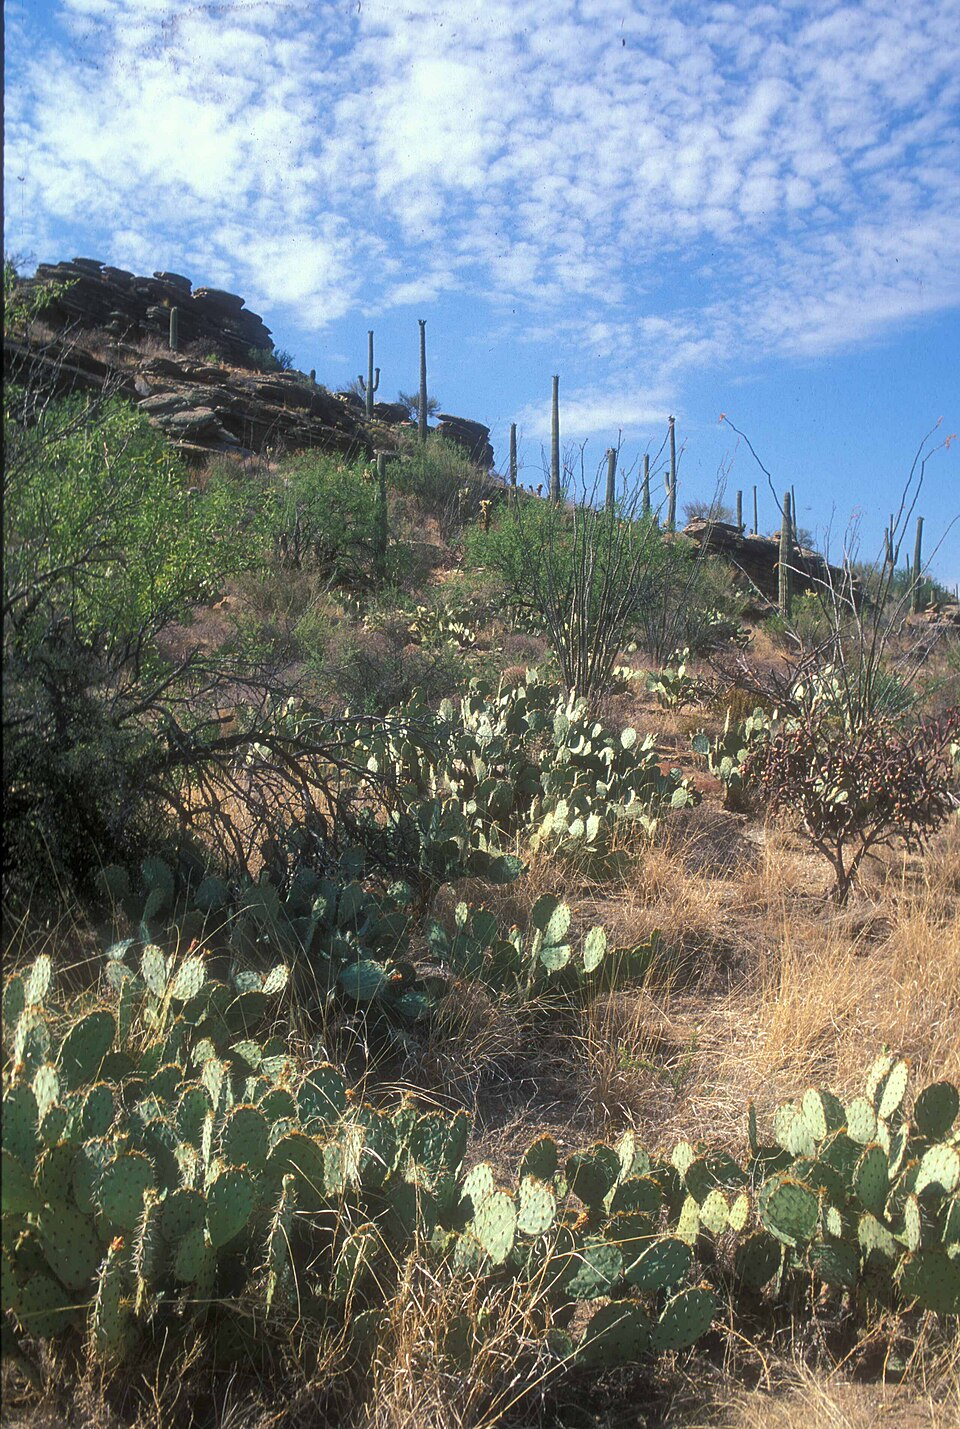
\includegraphics[height=3.6cm]{images/book1/g5-sonoran-desert.jpg}\quad
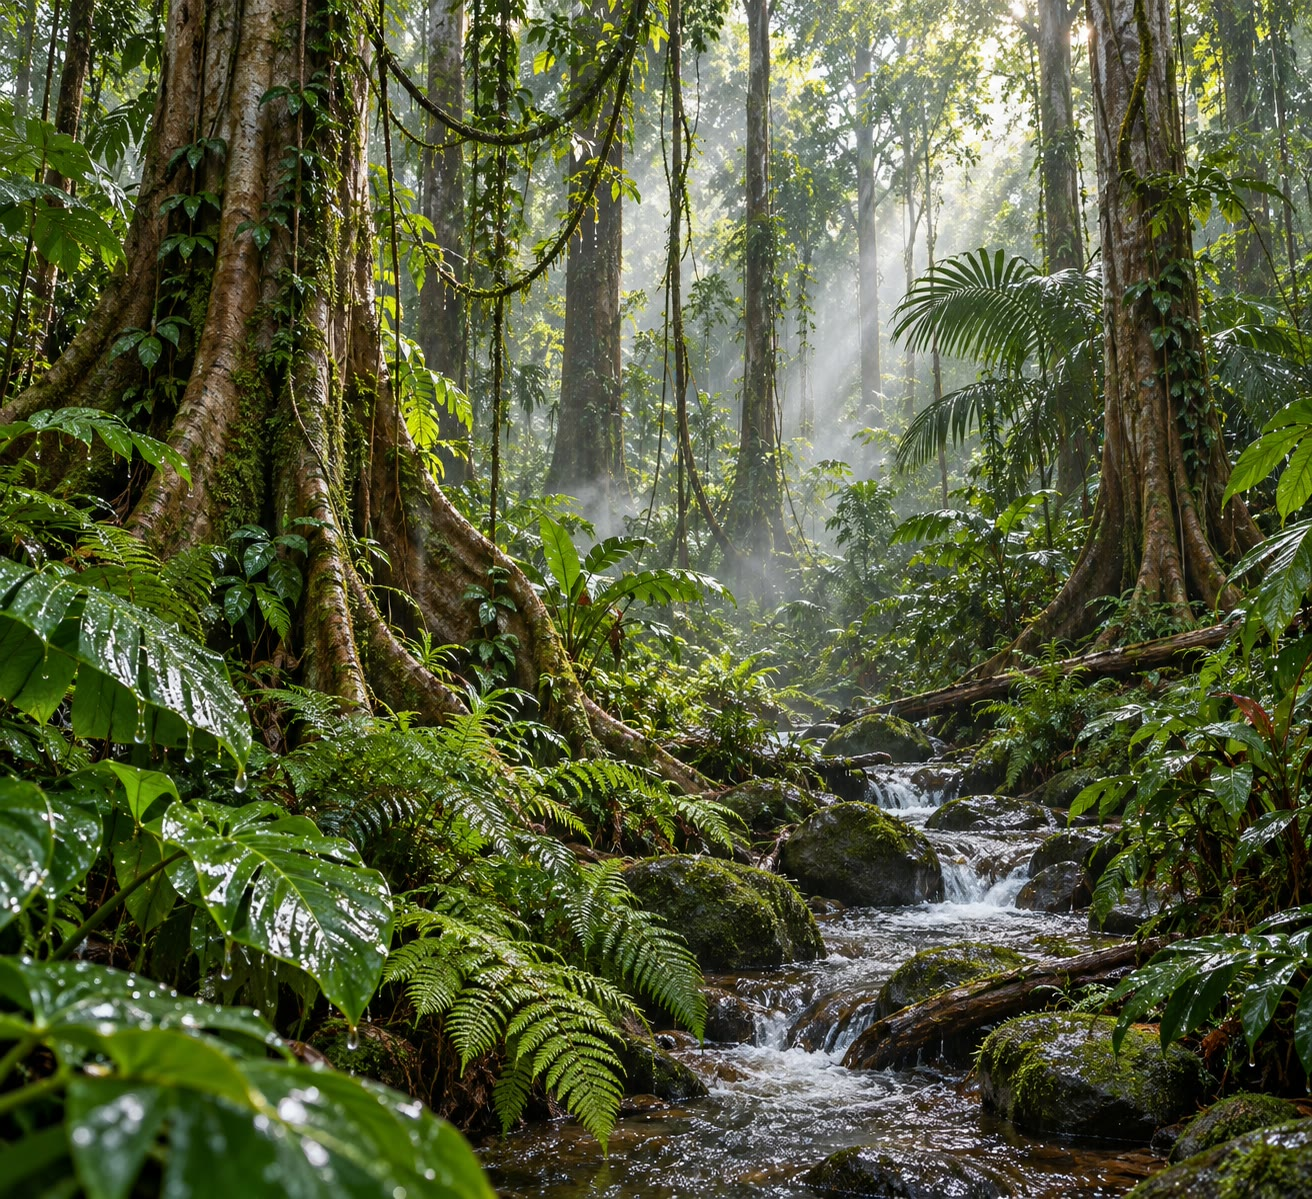
\includegraphics[height=3.6cm]{images/book1/ai/g5-rainforest.jpg}\quad
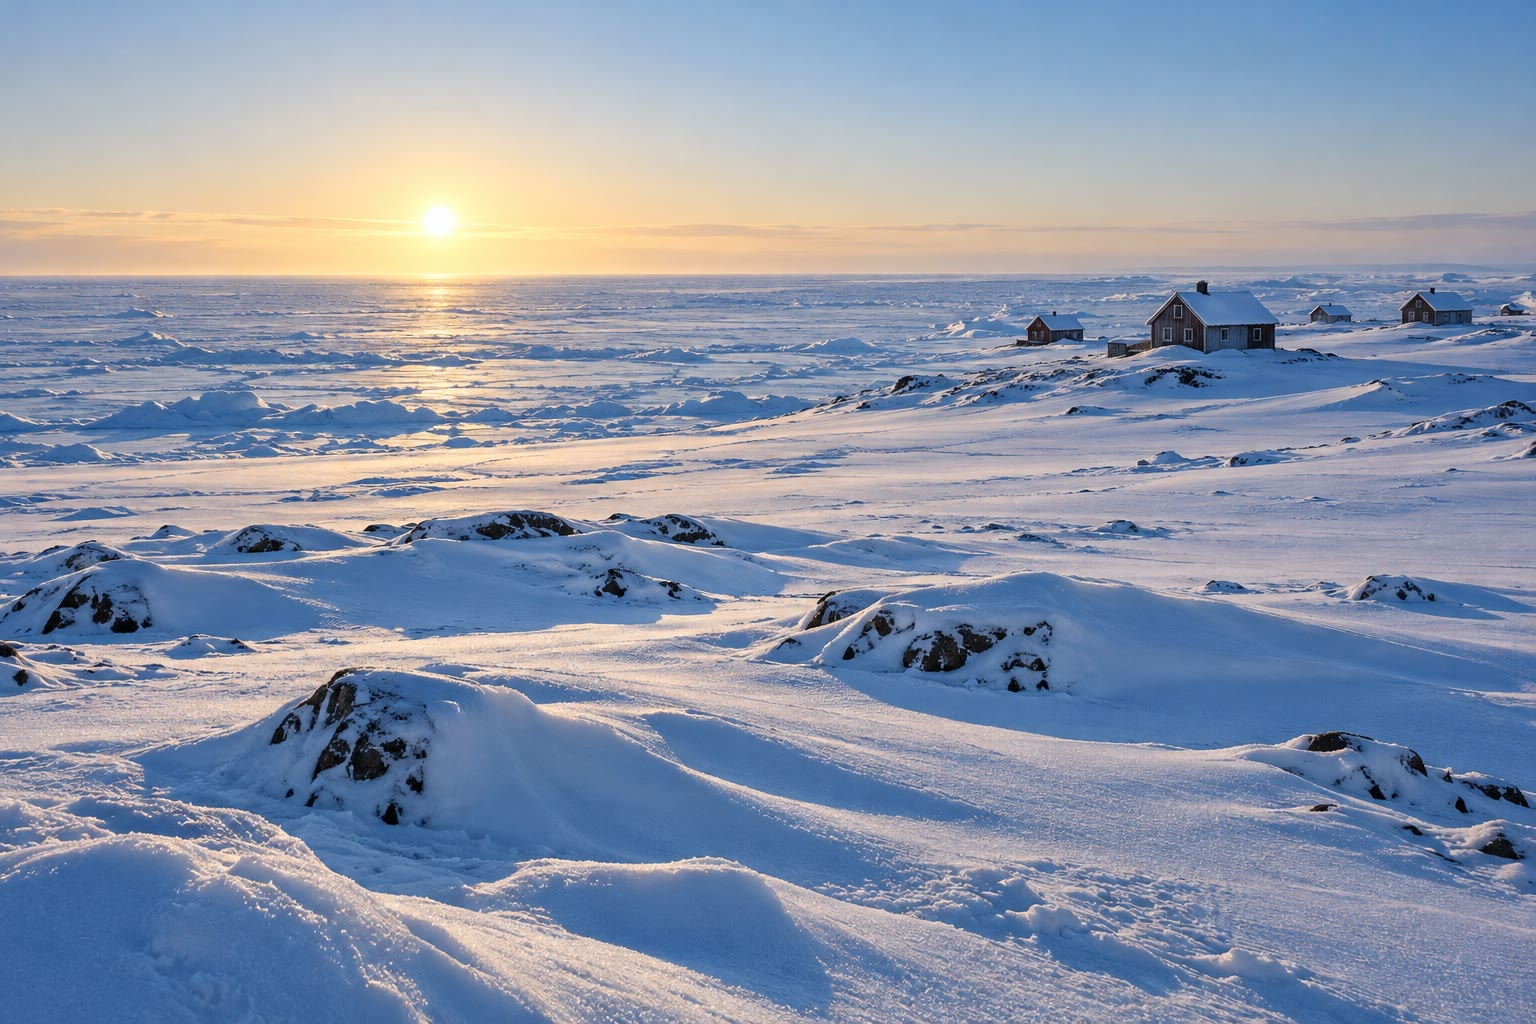
\includegraphics[height=3.6cm]{images/book1/ai/g5-polar-tundra.jpg}

{\small Trois \omterm{def:g5:weather-and-climate:climate}{climats} extrêmes. À gauche~: le \omterm{def:g5:weather-and-climate:desert}{désert} de Sonora en Arizona,
le \omterm{def:g5:weather-and-climate:desert}{désert} de Phoenix, avec de grands cactus saguaros et des figuiers de
Barbarie, qui stockent l'eau dans leurs tiges épaisses (photographie~:
U.S. National Park Service, Saguaro National Park, domaine public). Au
milieu~: l'intérieur d'une \omterm{def:g5:weather-and-climate:rainforest}{forêt tropicale humide} après une averse. À
droite~: une \omterm{def:g1:landscapes-around-us:water}{côte} polaire en hiver, avec une \omterm{def:g2:water-on-earth:ocean}{mer} gelée et un Soleil bas à
midi.}
% ledger: nps:sonoran-desert
\end{omfigure}

\paragraph{Le climat tempéré.} Seattle est entre les deux~: sa courbe monte
en été et descend en hiver, mais jamais de beaucoup~; il pleut assez,
surtout en automne et en hiver. C'est un \omterm{def:g5:weather-and-climate:climate}{climat} tempéré~: ni grandes
chaleurs, ni grands froids.

\paragraph{Le climat polaire.} À Utqiaġvik, la courbe rouge reste sous
0~$^\circ$C pendant huit mois de l'année~; en février, la moyenne est de
24 degrés sous zéro. Même en juillet, le mois le plus chaud, il ne fait
qu'environ 5 degrés.
% ledger: data:b1-noaa-normals

\section{Zones chaude, tempérées et froides}

Pourquoi fait-il chaud près de l'\omterm{def:g3:continents-and-oceans:equator}{équateur} et froid près des \omterm{def:g3:continents-and-oceans:poles}{pôles}~? À cause
du Soleil. Près de l'\omterm{def:g3:continents-and-oceans:equator}{équateur}, le Soleil de midi est haut dans le ciel
toute l'année~: sa lumière tombe presque à la verticale et chauffe
fortement le sol. Près des \omterm{def:g3:continents-and-oceans:poles}{pôles}, le Soleil reste toujours bas~: sa lumière
arrive en oblique, étalée sur une grande surface, et elle chauffe peu. En
hiver, là-bas, le Soleil peut même ne pas se lever du tout.

Deux paires de lignes qui font le tour du \omterm{def:g3:continents-and-oceans:globe}{globe} partagent la Terre en \omterm{def:g5:weather-and-climate:climate-zone}{zones climatiques}.

\begin{definition}[Tropiques et cercles polaires]\label{def:g5:weather-and-climate:tropics}
Les deux \emph{tropiques}\index{tropique} sont les lignes qui font le tour
du \omterm{def:g3:continents-and-oceans:globe}{globe}, l'une au nord et l'autre au sud de l'\omterm{def:g3:continents-and-oceans:equator}{équateur}, et qui marquent
jusqu'à quelle distance de l'\omterm{def:g3:continents-and-oceans:equator}{équateur} le Soleil de midi peut se trouver
exactement à la verticale~: le tropique du Cancer au nord, le tropique du
Capricorne au sud. Les deux
\emph{cercles polaires}\index{cercle polaire} sont les lignes qui font le
tour du \omterm{def:g3:continents-and-oceans:globe}{globe}, près des \omterm{def:g3:continents-and-oceans:poles}{pôles}, au-delà desquelles, au cœur de l'hiver, le
Soleil ne se lève pas pendant au moins un jour, et au cœur de l'été, il ne
se couche pas~: le cercle polaire arctique au nord, le cercle polaire
antarctique au sud.
\end{definition}

L'inclinaison de l'axe de la Terre décide de l'emplacement de ces lignes.

\begin{definition}[Zones climatiques]\label{def:g5:weather-and-climate:climate-zone}
La Terre est partagée en trois sortes de
\emph{zone climatique}\index{zone climatique}~: la \emph{zone chaude},
entre les deux \omterm{def:g5:weather-and-climate:tropics}{tropiques}, autour de l'\omterm{def:g3:continents-and-oceans:equator}{équateur}~; les deux
\emph{zones tempérées}, entre un \omterm{def:g5:weather-and-climate:tropics}{tropique} et un \omterm{def:g5:weather-and-climate:tropics}{cercle polaire}, où les étés
et les hivers diffèrent~; et les deux \emph{zones froides}, au-delà des
\omterm{def:g5:weather-and-climate:tropics}{cercles polaires}, autour des \omterm{def:g3:continents-and-oceans:poles}{pôles}.
\end{definition}

\begin{omfigure}
\begin{tikzpicture}
\begin{axis}[ommap, width=\linewidth, xtick=\empty, ytick=\empty, grid=none,
    axis background/.style={fill=white}, clip=true]
  \addplot[fill=orange!35, draw=none] table {figdata/out/grade-5-climate_zones-hot.dat};
  \addplot[fill=green!20, draw=none] table {figdata/out/grade-5-climate_zones-temperate.dat};
  \addplot[fill=cyan!20, draw=none] table {figdata/out/grade-5-climate_zones-cold.dat};
  \addplot[fill=black!25, fill opacity=0.8, draw=black!60, line width=0.2pt]
    table {figdata/out/shared-geo-land.dat};
  \addplot[black!70, dashed, line width=0.5pt] table {figdata/out/grade-5-climate_zones-lines.dat};
  \draw[black!70, line width=0.6pt] (axis cs:-180,0) -- (axis cs:180,0);
  \addplot[only marks, mark=*, mark size=1.8pt, red!80!black]
    table[x=lon, y=lat] {figdata/out/grade-5-climate_zones-stations.dat};
  \begin{scope}[every node/.style={font=\scriptsize, fill=white, fill opacity=0.75,
      text opacity=1, inner sep=1pt}]
    \node[anchor=west] at (axis cs:-107,33.4) {Phoenix};
    \node[anchor=east] at (axis cs:-158,19.7) {Hilo};
    \node[anchor=west] at (axis cs:-117,47.4) {Seattle};
    \node[anchor=west] at (axis cs:-151,73.5) {Utqiaġvik};
  \end{scope}
  \begin{scope}[every node/.style={font=\scriptsize\bfseries, align=center,
      fill=white, fill opacity=0.7, text opacity=1, inner sep=1pt}]
    \node at (axis cs:-5,83) {zone froide};
    \node at (axis cs:-40,40) {zone tempérée};
    \node at (axis cs:-25,-8) {zone chaude};
    \node at (axis cs:95,-45) {zone tempérée};
    \node at (axis cs:-60,-80) {zone froide};
  \end{scope}
\end{axis}
\end{tikzpicture}

{\small Les \omterm{def:g5:weather-and-climate:climate-zone}{zones climatiques}. De haut en bas, les lignes en tirets sont le
\omterm{def:g5:weather-and-climate:tropics}{cercle polaire} arctique, le \omterm{def:g5:weather-and-climate:tropics}{tropique} du Cancer, le \omterm{def:g5:weather-and-climate:tropics}{tropique} du Capricorne
et le \omterm{def:g5:weather-and-climate:tropics}{cercle polaire} antarctique~; la ligne continue est l'\omterm{def:g3:continents-and-oceans:equator}{équateur}. Les
points rouges sont les quatre villes des \omterm{def:g5:weather-and-climate:climate-chart}{diagrammes climatiques} ci-dessus.}
% ledger: earth:obliquity, data:b1-noaa-normals
\end{omfigure}

Les zones donnent une première image, grossière. À l'intérieur de chacune,
bien d'autres choses modifient le \omterm{def:g5:weather-and-climate:climate}{climat}~: la distance d'un lieu à la \omterm{def:g2:water-on-earth:ocean}{mer},
son \omterm{def:g4:world-physical-map:altitude}{altitude}, l'origine de ses vents. Tu les découvriras dans les classes
suivantes.

\begin{remark}[Phoenix et les zones]\label{rem:g5:weather-and-climate:phoenix}
Sur la \omterm{def:g2:drawing-to-map:map}{carte} des zones, Phoenix se trouve un peu au nord du \omterm{def:g5:weather-and-climate:tropics}{tropique} du
Cancer, dans la zone tempérée, et pourtant c'est un \omterm{def:g5:weather-and-climate:desert}{désert} chaud. Les zones
ne sont qu'une première image, grossière~: beaucoup des grands \omterm{def:g5:weather-and-climate:desert}{déserts}
chauds se trouvent près des \omterm{def:g5:weather-and-climate:tropics}{tropiques}, en bordure de la zone chaude, et tu
apprendras pourquoi au \cref{ch:g8:winds-global-circulation}.
\end{remark}

\section{Exercices}

\begin{exercise}[$\star$]\label{exo:g5:weather-and-climate:1}
Temps ou \omterm{def:g5:weather-and-climate:climate}{climat}~?
\begin{enumerate}
  \item[(a)] Il \omterm{def:g4:clouds-rain-snow:precipitation}{neige} à Utqiaġvik ce matin.
  \item[(b)] À Phoenix, les étés sont très chauds et secs.
  \item[(c)] Hier après-midi, un vent fort a soufflé sur Seattle.
  \item[(d)] À Hilo, il pleut beaucoup chaque mois de l'année.
\end{enumerate}
\end{exercise}

\begin{exercise}[$\star$]\label{exo:g5:weather-and-climate:2}
Qu'est-ce que le \omterm{def:g5:weather-and-climate:climate}{climat} d'un lieu~? Sur combien d'années les météorologues
font-ils la moyenne de leurs mesures pour le décrire~?
\end{exercise}

\begin{exercise}[$\star$]\label{exo:g5:weather-and-climate:3}
Sur le \omterm{def:g5:weather-and-climate:climate-chart}{diagramme climatique} de Seattle, quel est le mois le plus froid~?
Quel est le mois le plus humide~? La température descend-elle parfois sous
0~$^\circ$C~?
\end{exercise}

\begin{exercise}[$\star$]\label{exo:g5:weather-and-climate:4}
Sur le \omterm{def:g5:weather-and-climate:climate-chart}{diagramme climatique} d'Utqiaġvik, quel est le mois le plus chaud~?
Un mois dépasse-t-il 10~$^\circ$C~?
\end{exercise}

\begin{exercise}[$\star$]\label{exo:g5:weather-and-climate:5}
Dans quelle \omterm{def:g5:weather-and-climate:climate-zone}{zone climatique} se trouve chacun de ces lieux~: l'\omterm{def:g3:continents-and-oceans:equator}{équateur}~; le
\omterm{def:g3:continents-and-oceans:poles}{pôle Nord}~; un lieu à mi-chemin entre l'\omterm{def:g3:continents-and-oceans:equator}{équateur} et le \omterm{def:g3:continents-and-oceans:poles}{pôle Sud}~?
\end{exercise}

\begin{exercise}[$\star$]\label{exo:g5:weather-and-climate:6}
Utilise la \omterm{def:g2:drawing-to-map:map}{carte} des zones. Dans quelle \omterm{def:g5:weather-and-climate:climate-zone}{zone climatique} se trouve chacune
des quatre villes~: Phoenix, Hilo, Seattle, Utqiaġvik~?
\end{exercise}

\begin{exercise}[$\star\star$]\label{exo:g5:weather-and-climate:7}
Voici la \omterm{def:g4:clouds-rain-snow:precipitation}{pluie} moyenne de chaque mois à Seattle, en millimètres, arrondie à
l'unité~:
\begin{center}
\begin{tabular}{|*{12}{c|}}
\hline
J & F & M & A & M & J & J & A & S & O & N & D\\
\hline
147 & 96 & 106 & 81 & 48 & 37 & 15 & 25 & 41 & 99 & 160 & 145\\
\hline
\end{tabular}
\end{center}
Combien de \omterm{def:g4:clouds-rain-snow:precipitation}{pluie} tombe-t-il à Seattle sur une année entière~? Combien en
tombe-t-il pendant les trois mois de décembre, janvier et février~?
% ledger: data:b1-noaa-normals
\end{exercise}

\begin{exercise}[$\star\star$]\label{exo:g5:weather-and-climate:8}
À Phoenix, la température moyenne est de 14~$^\circ$C en janvier et de
35~$^\circ$C en juillet. À Hilo, elle est de 22~$^\circ$C en janvier et de
25~$^\circ$C en juillet. Calcule la différence entre juillet et janvier
dans chaque ville. Où les saisons font-elles le plus varier la
température~?
% ledger: data:b1-noaa-normals
\end{exercise}

\begin{exercise}[$\star\star$]\label{exo:g5:weather-and-climate:9}
Voici les moyennes d'une ville imaginaire.
\begin{center}
\begin{tabular}{|l|*{12}{c|}}
\hline
mois & J & F & M & A & M & J & J & A & S & O & N & D\\
\hline
température ($^\circ$C) & 27 & 27 & 28 & 28 & 28 & 27 & 27 & 27 & 27 & 27 & 27 & 27\\
\hline
\omterm{def:g4:clouds-rain-snow:precipitation}{pluie} (mm) & 250 & 230 & 280 & 290 & 260 & 180 & 170 & 160 & 190 & 230 & 250 & 260\\
\hline
\end{tabular}
\end{center}
Est-ce un \omterm{def:g5:weather-and-climate:desert}{désert}, une \omterm{def:g5:weather-and-climate:rainforest}{forêt tropicale humide}, un \omterm{def:g5:weather-and-climate:climate}{climat} tempéré ou un
\omterm{def:g5:weather-and-climate:climate}{climat} polaire~? Donne deux raisons. Dans quelle zone la ville a-t-elle le
plus de chances de se trouver~?
\end{exercise}

\begin{exercise}[$\star\star$]\label{exo:g5:weather-and-climate:10}
Reprends les deux cartes postales du début du chapitre, envoyées la même
semaine de janvier. Donne deux explications différentes du fait que des
enfants peuvent jouer sur une plage ensoleillée à un endroit, pendant que
d'autres font un bonhomme de \omterm{def:g4:clouds-rain-snow:precipitation}{neige} ailleurs.
\end{exercise}

\begin{exercise}[$\star\star\star$]\label{exo:g5:weather-and-climate:11}
Noor dit~: «~Phoenix et Seattle sont toutes les deux dans la zone tempérée,
donc elles ont forcément le même \omterm{def:g5:weather-and-climate:climate}{climat}.~» Utilise les \omterm{def:g5:weather-and-climate:climate-chart}{diagrammes
climatiques} pour montrer qu'elle a tort~: compare leurs températures et
leurs \omterm{def:g4:clouds-rain-snow:precipitation}{pluies}. Dis ensuite ce que les \omterm{def:g5:weather-and-climate:climate-zone}{zones climatiques} nous apprennent, et
ce qu'elles ne nous apprennent pas.
\end{exercise}
